\documentclass[conference,a4paper]{IEEEtran}
\IEEEoverridecommandlockouts

% ============================================================================
% IEEE Conference Manuscript for ICEIB (https://www.iceib.asia/)
% Format: A4, Double-Column, Single-Spaced, No Page Numbers / Headers / Footers
% Target Length: <= 6 Pages (IEEE Xplore Track)
% ============================================================================

\usepackage{cite}
\usepackage{amsmath,amssymb,amsfonts}
\usepackage{algorithm}
\usepackage{algorithmic}
\usepackage{graphicx}
\usepackage{textcomp}
\usepackage{xcolor}
\usepackage{booktabs}
\usepackage{array}
\usepackage{tabularx}
\usepackage{placeins}
\usepackage{url}
\expandafter\def\expandafter\UrlBreaks\expandafter{\UrlBreaks\do\~}
\usepackage{tikz}
\usetikzlibrary{arrows.meta, positioning, shapes.geometric}

% Suppress page numbers, headers, and footers per ICEIB / IEEE submission rules
\pagestyle{empty}

\def\BibTeX{{\rm B\kern-.05em{\sc i\kern-.025em b}\kern-.08em
    T\kern-.1667em\lower.7ex\hbox{E}\kern-.125emX}}

\begin{document}

\title{An Evidence-Grounded Chinese-Language Task Agent and Specification-Driven Architecture for Indoor Navigation With TurtleBot3 Burger}

\author{
\IEEEauthorblockN{Cheng-Hao Hsiao}
\IEEEauthorblockA{
\textit{Department of Electrical Engineering}\\
\textit{National Chung Hsing University}\\
Taichung, Taiwan\\
hank050392@gmail.com
}
}

\maketitle
\thispagestyle{empty}

\begin{abstract}
Natural-language interfaces simplify indoor robot operation, yet translating an utterance into a navigation goal does not establish that the destination is unambiguous, the robot is ready, or the mission has physically succeeded. This paper presents an evidence-grounded Chinese-language task agent and specification-driven architecture for indoor navigation on TurtleBot3 Burger using ROS~2 Humble and Nav2. The design separates semantic interpretation, constrained tool execution, Nav2 motion control, and evidence-backed reporting across eight modules. A large language model produces schema-constrained intents, while a registered landmark catalog, strict parameter allowlists, and domain checks prevent arbitrary coordinate generation and unsafe dispatch. When references are ambiguous, the agent requests clarification prior to dispatch; before execution, it verifies localization, coordinate transform (TF), LiDAR scan freshness, and path feasibility. During execution, it enforces single-mission ownership, cancellation priority, at most one agent-level retry, and independent verification of endpoint tolerances and physical stopping. Using OpenSpec~2.0.0, the verified offline contract baseline is separated from pending runtime capabilities. An offline Python prototype passes all nine unit tests in 0.001~s, while ROS~2 Humble/Nav2 integration and a 60-command evaluation protocol comparing fixed menus (B0), direct parsing (B1), and the full agent (B2) remain planned for empirical validation.
\end{abstract}

\begin{IEEEkeywords}
Indoor navigation, task agents, large language models, TurtleBot3, ROS~2 Humble, specification-driven development.
\end{IEEEkeywords}

\section{Introduction}

In indoor laboratory settings, non-expert users expect to command mobile robots with natural-language instructions such as ``go beside the desk'' or ``go to the doorway'' in Traditional Chinese rather than raw map coordinates. While ROS~2 Nav2~\cite{b4} handles global planning, local trajectory control, and behavior-tree recovery once a valid pose is given, a dependable task interface must answer three operational questions: (i) which registered physical location matches the request, (ii) whether localization, sensing, and path availability justify dispatching a goal, and (iii) what terminal state actually occurred based on observable evidence.

Bridging natural language and physical navigation exposes coupled semantic and cyber-physical failure modes. SayCan~\cite{b2} demonstrates the need to ground language plans in physical affordances, while Pollini et al.~\cite{b3} show that integrating large language models (LLMs) with ROS~2 introduces measurable communication latency. On a compact differential-drive TurtleBot3 Burger~\cite{b8}, a single Chinese phrase (e.g., requesting ``go to the doorway'') may match multiple entrances, an unknown room name may induce coordinate hallucination, and stale LiDAR scans or transform (TF) dropouts can invalidate execution even for valid targets. Crucially, structured intent parsing, Nav2 goal acceptance, and physical arrival are distinct events requiring independent verification.

Given a Chinese request $Q$, a versioned landmark registry $K$, an active 2D occupancy map $M$, and a timestamped robot status vector $S$, the agent must decide among clarifying, rejecting, dispatching, canceling, or reporting terminal status such that every action or status claim is backed by traceable evidence $E$. Linguistic plausibility must never replace ROS~2 action results or fresh sensor observations. Accordingly, this work addresses three research questions (RQs):
\begin{itemize}
    \item \textbf{RQ1:} Does interactive clarification reduce inappropriate dispatches caused by destination ambiguity and unknown landmarks?
    \item \textbf{RQ2:} Do pre-dispatch freshness and path-feasibility checks reduce erroneous goal dispatches under sensor, localization, or reachability faults?
    \item \textbf{RQ3:} Does evidence-grounded reporting improve state consistency between robot outcomes and user reports, and what latency overhead does it incur?
\end{itemize}

This work is scoped to a single TurtleBot3 Burger on one indoor floor with a pre-built 2D map and manually registered landmarks, targeting ROS~2 Humble. It excludes object recognition, manipulation, multi-robot coordination, reinforcement learning (RL) training, and novel path-planning algorithms. Our main contributions are:
\begin{enumerate}
    \item \textbf{Constrained Chinese Task Interface:} An eight-module architecture binding LLM outputs to a four-intent schema and landmark allowlist while clarifying ambiguous requests before dispatch.
    \item \textbf{State-Aware Mission Lifecycle:} Single-mission ownership, cancellation priority, pre-dispatch gating, at most one agent-level retry, and separate verification of arrival tolerances and physical stopping.
    \item \textbf{OpenSpec Specification Separation:} Formal separation between the verified \path{offline-contract} baseline and pending runtime capabilities (\path{navigation-mission}, \path{mission-evaluation}) in OpenSpec~2.0.0.
    \item \textbf{Evaluation Protocol and Offline Verification:} A three-baseline, two-ablation design over 60 template-split Chinese commands and four scenarios, paired with an offline Python prototype passing nine contract tests.
\end{enumerate}

The paper is organized as follows. Section~II reviews related work and the integration gap. Section~III presents domain principles and trade-offs. Section~IV details the architecture, flowchart, algorithm, tool contracts, and OpenSpec workflow. Section~V defines the evaluation protocol. Section~VI reports current offline verification results, and Section~VII concludes with limitations and future work.

\section{Related Work}

\subsection{Language Agents and Action Feasibility}

ReAct~\cite{b1} alternates reasoning traces with tool actions and environmental observations across interactive benchmarks (HotpotQA, FEVER, ALFWorld, WebShop). Although our agent borrows this observe--validate--act pattern, benchmark accuracy does not establish physical robot safety. SayCan~\cite{b2} pairs LLM planning with skill value functions to constrain plans by affordances; instead of learned value functions, we enforce deterministic constraints via a landmark catalog, JSON schema validation, and Nav2 readiness checks.

Pollini et al.~\cite{b3} integrated ChatGPT with ROS~2 in Gazebo and reported reduced command-processing latency, motivating our measurement of parse, dispatch, and reporting latencies ($p_{50}$ and $p_{95}$). However, their simulation study does not address Traditional Chinese landmark disambiguation, explicit mid-mission stopping confirmation, or stale-sensor fault injection on TurtleBot3 Burger.

\subsection{Modular Navigation, Mapping, and Evaluation}

The Marathon~2~\cite{b4} established Nav2 as a modular ROS~2 navigation stack coordinating planning, control, and recovery via behavior trees, while SLAM Toolbox~\cite{b5} provides 2D graph-based SLAM and localization. Both supply the spatial substrate beneath our agent, yet neither resolves natural-language ambiguity nor audits task-level reporting consistency.

To benchmark constrained navigation, the BARN Challenge~\cite{b6, b12} evaluates classical and learned planners in cluttered obstacle courses, retaining failures across repeated trials. RoboRAN~\cite{b7} provides a unified RL navigation framework with sim-to-real deployment. Rather than training RL policies or transferring scores across mismatched platforms, we fix the Nav2 substrate and adopt multi-scenario failure retention to isolate task-layer gains. Official TurtleBot3 and Nav2 documentation~\cite{b8, b9, b10, b11} informs footprint calibration, costmap tuning, Humble Simple Commander integration, and low-latency collision monitoring.

\begin{table}[!t]
\caption{Comparison of Representative Related Work and Applicability Boundaries}
\label{tab:related_work}
\centering
\scriptsize
\setlength{\tabcolsep}{3pt}
\begin{tabularx}{\columnwidth}{@{} >{\raggedright\arraybackslash}p{0.9cm} >{\raggedright\arraybackslash}p{1.85cm} >{\raggedright\arraybackslash}p{2.25cm} >{\raggedright\arraybackslash}X @{}}
\toprule
\textbf{Ref.} & \textbf{Focus} & \textbf{Adopted Element} & \textbf{Boundary / Gap Addressed} \\
\midrule
\cite{b1} & ReAct tool loop & Action--observation feedback & Text/QA benchmarks; no ROS~2 or physical safety proof \\
\cite{b2} & SayCan affordances & Feasibility-constrained planning & Uses learned skills; replaced by allowlists \& checks \\
\cite{b3} & LLM + ROS~2 latency & Interaction latency logging & Gazebo setup; lacks Chinese ambiguity \& fault checks \\
\cite{b4} & Nav2 behavior trees & Modular planning and recovery & No Chinese NLU, clarification, or evidence audit \\
\cite{b5} & SLAM Toolbox & 2D mapping and localization & Spatial backend only; no semantic task planning \\
\cite{b6, b12} & BARN Challenge & Constrained trials \& failure retention & Different platforms/scales; needs Burger calibration \\
\cite{b7} & RoboRAN RL & Cross-scenario evaluation & RL framework; our baseline fixes Nav2 \\
\bottomrule
\end{tabularx}
\end{table}

\subsection{Research Gap}

As summarized in Table~\ref{tab:related_work}, prior work establishes language-action loops and modular ROS~2 navigation independently. Our motivation is therefore not that language-guided navigation is unexplored, but to quantify whether, on a fixed ROS~2 Humble TurtleBot3 Burger and Nav2 stack, Chinese landmark clarification, pre-dispatch gating, and evidence-grounded reporting improve handling and report consistency---and at what latency cost.

\section{Domain Principles and Design Trade-Offs}

The architecture is governed by seven domain rules (\texttt{K01}--\texttt{K07}) in Table~\ref{tab:domain_rules}, derived from five engineering principles and three architectural trade-offs.

\begin{table}[!t]
\caption{Domain Knowledge Rules and Architectural Impact}
\label{tab:domain_rules}
\centering
\scriptsize
\setlength{\tabcolsep}{3pt}
\begin{tabularx}{\columnwidth}{@{} >{\raggedright\arraybackslash}p{0.65cm} >{\raggedright\arraybackslash}p{2.45cm} >{\raggedright\arraybackslash}p{1.05cm} >{\raggedright\arraybackslash}X @{}}
\toprule
\textbf{ID} & \textbf{Rule} & \textbf{Source} & \textbf{System Design Impact} \\
\midrule
\texttt{K01} & Localization is uncertain; odometry $\neq$ truth & \cite{b4, b5} & Check pose age and TF; verify final pose tolerance \\
\texttt{K02} & 2D LiDAR has planar blind-spot limits & \cite{b8} & Treat stale/missing scans as \texttt{NOT\_READY}, not free space \\
\texttt{K03} & Planning must respect robot footprint & \cite{b9} & Calibrate Burger footprint; never shrink to force arrival \\
\texttt{K04} & Linguistic plausibility $\neq$ feasibility & \cite{b2} & Enforce landmark allowlist, schema, and path checks \\
\texttt{K05} & Action completion $\neq$ mission success & \cite{b10} & Read terminal result; separate \texttt{CANCELED} and \texttt{ARRIVED} \\
\texttt{K06} & Multi-scenario tests beat single demos & \cite{b6, b7, b12} & Fix baselines, keep failures, report intervals \\
\texttt{K07} & Low-latency stop cannot wait for LLM & \cite{b11} & Keep Nav2 Collision Monitor independent of LLMs \\
\bottomrule
\end{tabularx}
\end{table}

\subsection{Five Core Engineering Principles}

\subsubsection{Localization Is an Uncertain Estimate (\texttt{K01})}
Wheel slip and repetitive corridors cause odometry drift. Before dispatch, the agent checks TF integrity (\texttt{map}~$\rightarrow$~\texttt{odom}~$\rightarrow$~\texttt{base\_link}) and pose freshness; upon completion, it verifies final pose tolerances rather than relying solely on encoder integration or a single covariance threshold.

\subsubsection{Sensor Blindness Is Not Safety (\texttt{K02})}
A 2D planar LiDAR misses overhangs outside its scan plane, and driver dropouts or infinite/zero readings require explicit handling. Stale or missing scan feeds block dispatch and trigger fault cancellation in motion.

\subsubsection{Footprint and Kinematic Feasibility (\texttt{K03})}
Nav2 costmap inflation and physical chassis geometry determine narrow-doorway traversability~\cite{b9}. Footprint settings are calibrated to the physical Burger chassis and never reduced to inflate arrival rates.

\subsubsection{Layered Semantics and Real-Time Control (\texttt{K04}, \texttt{K07})}
The LLM-backed agent handles intent parsing, clarification, and reporting, while Nav2 computes paths and velocities. The LLM invokes only allowlisted tools with registered landmarks and cannot emit wheel velocities or modify safety parameters. Local obstacle stopping (e.g., Nav2 Collision Monitor~\cite{b11}) operates independently of remote LLM inference.

\subsubsection{Reliability via Repeated Evaluation (\texttt{K05}, \texttt{K06})}
Single successful runs do not prove robustness. Evaluation separates parsing, navigation execution, and report consistency across multiple scenarios while retaining all failures and timeouts.

\subsection{Three Architectural Trade-Offs}

\subsubsection{Modular Nav2 vs. End-to-End RL}
Modular stacks allow transparent fault attribution~\cite{b4}, whereas RL policies learn sensor-to-action mappings directly~\cite{b7}. To isolate task-layer agent decisions, we fix Nav2 as the shared motion layer and defer RL comparison.

\subsubsection{Pre-Built Map vs. Mapless Navigation}
Pre-built maps from SLAM Toolbox~\cite{b5} anchor named indoor landmarks and detect global deadlocks, whereas mapless navigation avoids prior mapping~\cite{b6}. We adopt a pre-built map with Nav2's live local costmap for unexpected obstacles and clarify unregistered names instead of guessing coordinates.

\subsubsection{Conservative Clearance vs. Traversal Efficiency}
Conservative speeds and inflation margins tolerate drift and latency but can reject narrow passages~\cite{b6, b9}. We fix one calibrated conservative Nav2 configuration across all baselines and prohibit runtime margin mutation by the agent.

\section{Proposed System Architecture and Specification-Driven Workflow}

\subsection{Eight-Module System Architecture}

Fig.~\ref{fig:architecture} shows the eight-module architecture linking user commands to ROS~2 Humble and Nav2 execution:
\begin{enumerate}
    \item \textbf{User and Indoor Context:} Laboratory users issue Traditional Chinese mobility requests.
    \item \textbf{Input and Structured Parsing:} An LLM converts utterances into schema-constrained JSON intents and landmark IDs.
    \item \textbf{Planner and Task Agent:} Manages mission state, single-mission ownership, tool sequencing, and bounded retries.
    \item \textbf{Data Acquisition and Retrieval:} Reads \path{landmarks.json}, \path{domain_rules.md}, map, TF, pose, LiDAR scan, and Nav2 feedback.
    \item \textbf{Analytics Engine:} Tracks sensor age in ROS time, monotonic deadlines, path length, and evaluation metrics.
    \item \textbf{Domain Knowledge and Validation:} Enforces intent schemas, tool/landmark allowlists, map ID consistency, and safety rules.
    \item \textbf{Decision and Navigation Tools:} Resolves validated landmark IDs to \texttt{PoseStamped} goals in the \texttt{map} frame for Nav2.
    \item \textbf{Output and User Interaction:} Produces evidence-backed reports or clarification prompts and feeds replies back to Module~2.
\end{enumerate}

\begin{figure}[!t]
\centering
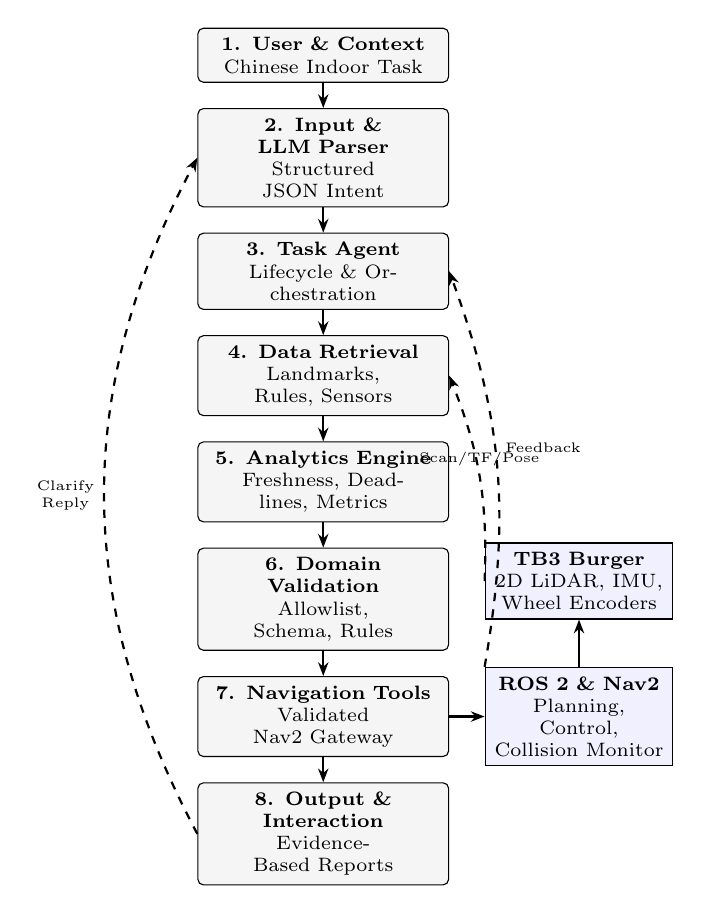
\begin{tikzpicture}[
    node distance=0.32cm and 0.42cm,
    box/.style={rectangle, draw=black, rounded corners=2pt, fill=gray!8, text width=2.95cm, align=center, font=\scriptsize, minimum height=0.52cm},
    hw/.style={rectangle, draw=black, fill=blue!6, text width=2.15cm, align=center, font=\scriptsize, minimum height=0.54cm},
    arr/.style={-{Stealth[scale=0.75]}, thick},
    darr/.style={-{Stealth[scale=0.75]}, dashed, thick}
]
\node[box] (u) {\textbf{1. User \& Context}\\Chinese Indoor Task};
\node[box, below=of u] (i) {\textbf{2. Input \& LLM Parser}\\Structured JSON Intent};
\node[box, below=of i] (a) {\textbf{3. Task Agent}\\Lifecycle \& Orchestration};
\node[box, below=of a] (d) {\textbf{4. Data Retrieval}\\Landmarks, Rules, Sensors};
\node[box, below=of d] (e) {\textbf{5. Analytics Engine}\\Freshness, Deadlines, Metrics};
\node[box, below=of e] (k) {\textbf{6. Domain Validation}\\Allowlist, Schema, Rules};
\node[box, below=of k] (t) {\textbf{7. Navigation Tools}\\Validated Nav2 Gateway};
\node[box, below=of t] (o) {\textbf{8. Output \& Interaction}\\Evidence-Based Reports};

\node[hw, right=0.45cm of t] (n) {\textbf{ROS~2 \& Nav2}\\Planning, Control,\\Collision Monitor};
\node[hw, above=0.6cm of n] (b) {\textbf{TB3 Burger}\\2D LiDAR, IMU,\\Wheel Encoders};

\draw[arr] (u) -- (i);
\draw[arr] (i) -- (a);
\draw[arr] (a) -- (d);
\draw[arr] (d) -- (e);
\draw[arr] (e) -- (k);
\draw[arr] (k) -- (t);
\draw[arr] (t) -- (o);
\draw[arr] (t) -- (n);
\draw[arr] (n) -- (b);
\draw[darr] (n.north west) to[bend right=15] node[right, font=\tiny, pos=0.55]{Feedback} (a.east);
\draw[darr] (b.west) to[bend right=12] node[above, font=\tiny]{Scan/TF/Pose} (d.east);
\draw[darr] (o.west) to[bend left=28] node[left, font=\tiny, align=center]{Clarify\\Reply} (i.west);
\end{tikzpicture}
\caption{Eight-module architecture of the proposed Chinese-language navigation agent with ROS~2 Humble/Nav2 and TurtleBot3 Burger feedback loops.}
\label{fig:architecture}
\end{figure}

\subsection{Mission Execution Flowchart and Core Algorithm}

Fig.~\ref{fig:flowchart} and Algorithm~\ref{alg:agent} formalize the mission lifecycle. Explicit cancellation takes priority over movement; concurrent movement requests receive \texttt{BUSY} until prior missions confirm termination. Validated navigation requests pass ambiguity checking (\texttt{CLARIFY}), schema/allowlist checks (\texttt{REJECTED}), sensor/TF/map readiness checks (\texttt{NOT\_READY}), and bounded path checks (\texttt{NO\_PATH}) before dispatch.

During execution, three safeguards prevent false success claims: (1) after Nav2's internal recovery ends in \texttt{FAILED}, the agent allows at most one redispatch only if fresh readiness and path checks pass (never after cancellation or timeout); (2) a confirmed cancel requires both terminal \texttt{CANCELED} action state and fresh motion observations satisfying stopping thresholds, otherwise returning \texttt{FAULT} (\path{stop_confirmed=false}) and blocking new tasks; and (3) \texttt{ARRIVED} requires Nav2 \texttt{SUCCEEDED} \emph{and} a fresh final pose within position and heading tolerances on the active map.

\begin{figure}[!t]
\centering
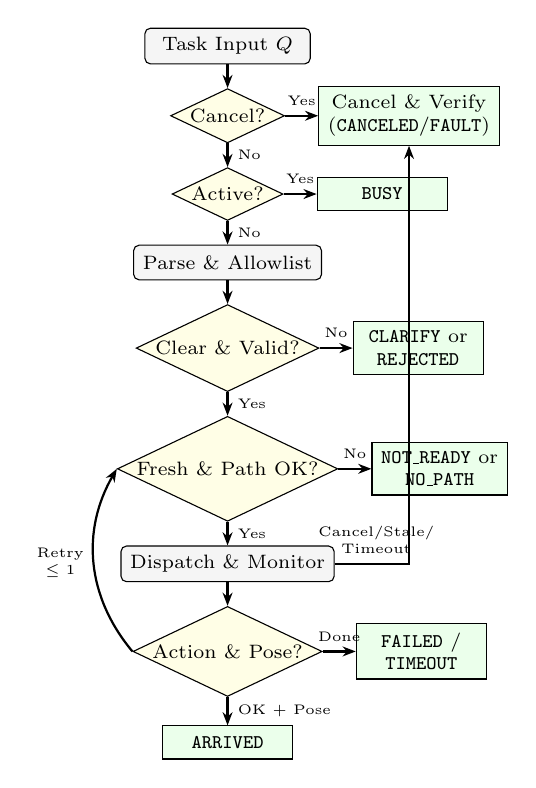
\begin{tikzpicture}[
    node distance=0.30cm and 0.38cm,
    proc/.style={rectangle, draw=black, rounded corners=2pt, fill=gray!8, align=center, font=\scriptsize, minimum width=2.1cm, minimum height=0.44cm},
    dec/.style={diamond, aspect=2.1, draw=black, fill=yellow!10, align=center, font=\scriptsize, inner sep=0.6pt},
    term/.style={rectangle, draw=black, fill=green!8, align=center, font=\scriptsize, minimum width=1.65cm, minimum height=0.42cm},
    arr/.style={-{Stealth[scale=0.72]}, thick}
]
\node[proc] (in) {Task Input $Q$};
\node[dec, below=of in] (c) {Cancel?};
\node[dec, below=of c] (b) {Active?};
\node[proc, below=of b] (p) {Parse \& Allowlist};
\node[dec, below=of p] (q) {Clear \& Valid?};
\node[dec, below=of q] (s) {Fresh \& Path OK?};
\node[proc, below=of s] (n) {Dispatch \& Monitor};
\node[dec, below=of n] (e) {Action \& Pose?};

\node[term, right=0.42cm of c] (x) {Cancel \& Verify\\(\texttt{CANCELED}/\texttt{FAULT})};
\node[term, right=0.42cm of b] (busy) {\texttt{BUSY}};
\node[term, right=0.42cm of q] (u) {\texttt{CLARIFY} or\\\texttt{REJECTED}};
\node[term, right=0.42cm of s] (f) {\texttt{NOT\_READY} or\\\texttt{NO\_PATH}};
\node[term, below=0.36cm of e] (arrv) {\texttt{ARRIVED}};
\node[term, right=0.42cm of e] (fail) {\texttt{FAILED} /\\\texttt{TIMEOUT}};

\draw[arr] (in) -- (c);
\draw[arr] (c) -- node[right, font=\tiny]{No} (b);
\draw[arr] (c) -- node[above, font=\tiny]{Yes} (x);
\draw[arr] (b) -- node[right, font=\tiny]{No} (p);
\draw[arr] (b) -- node[above, font=\tiny]{Yes} (busy);
\draw[arr] (p) -- (q);
\draw[arr] (q) -- node[right, font=\tiny]{Yes} (s);
\draw[arr] (q) -- node[above, font=\tiny]{No} (u);
\draw[arr] (s) -- node[right, font=\tiny]{Yes} (n);
\draw[arr] (s) -- node[above, font=\tiny]{No} (f);
\draw[arr] (n) -- (e);
\draw[arr] (e) -- node[right, font=\tiny]{OK + Pose} (arrv);
\draw[arr] (e) -- node[above, font=\tiny]{Done} (fail);
\draw[arr] (e.west) to[bend left=35] node[left, font=\tiny, align=center]{Retry\\$\le 1$} (s.west);
\draw[arr] (n.east) -| node[above, font=\tiny, pos=0.28, align=center]{Cancel/Stale/\\Timeout} (x.south);
\end{tikzpicture}
\caption{Mission control flowchart showing single-mission gating, pre-dispatch verification, bounded retry, and evidence-backed termination.}
\label{fig:flowchart}
\end{figure}

\begin{algorithm}[!htb]
\caption{Evidence-Grounded Indoor Navigation Agent}
\label{alg:agent}
\footnotesize
\begin{algorithmic}[1]
\REQUIRE Query $Q$, landmark registry $K$, robot status $S$
\ENSURE Mission result $R$ with traceable evidence $E$
\IF{$Q$ is an explicit cancel command}
    \STATE Cancel active goal; verify termination and stopping; \RETURN status
\ENDIF
\IF{another mission is active or unresolved}
    \RETURN \texttt{BUSY}
\ENDIF
\STATE Read $K$ and retrieve domain rules with source IDs
\STATE Parse $Q$ into schema-constrained intent via LLM
\IF{parsing fails or times out}
    \RETURN clarification or parsing error
\ENDIF
\IF{intent is ambiguous}
    \RETURN \texttt{CLARIFY} with candidate landmarks
\ENDIF
\STATE Validate tool name, landmark ID, and schema against allowlists
\IF{validation fails}
    \RETURN \texttt{REJECTED} without dispatching goal
\ENDIF
\STATE Check scan, localization, TF, and Nav2 lifecycle freshness
\IF{data are stale or checks fail}
    \RETURN \texttt{NOT\_READY} with observed evidence
\ENDIF
\STATE Resolve landmark ID to \texttt{PoseStamped} in \texttt{map} frame; check path
\IF{no valid path or path check timeout}
    \RETURN \texttt{NO\_PATH} without claiming arrival
\ENDIF
\STATE Dispatch validated goal via Nav2 adapter
\WHILE{monotonic mission deadline has not expired}
    \STATE Read Nav2 feedback and fresh status; append evidence $E$
    \IF{user cancels or status becomes unsafe/stale}
        \STATE Cancel goal; verify action state and stopping
        \RETURN \texttt{CANCELED} if confirmed, else \texttt{FAULT}
    \ENDIF
    \IF{navigation result is \texttt{SUCCEEDED}}
        \RETURN \texttt{ARRIVED} if final pose within tolerance, else \texttt{FAULT}
    \ENDIF
    \IF{navigation result is \texttt{FAILED} or \texttt{CANCELED}}
        \IF{\texttt{FAILED} and retry budget $\le 1$ and checks pass}
            \STATE Recheck path; redispatch once if valid path exists
        \ELSE
            \RETURN observed terminal result with evidence $E$
        \ENDIF
    \ENDIF
\ENDWHILE
\STATE Cancel goal; verify cancellation or flag unresolved state
\RETURN \texttt{TIMEOUT} with log IDs and stop-confirmation status
\end{algorithmic}
\end{algorithm}

\subsection{Tool Interfaces and Schema Contracts}

Table~\ref{tab:interfaces} defines the six allowlisted gateway tools. Only four JSON schemas are accepted: \texttt{navigate} (strictly \texttt{intent}, \texttt{landmark\_id}), \texttt{cancel} (\texttt{intent}), \texttt{clarify} (\texttt{intent}, non-empty \texttt{question}), and \texttt{reject} (\texttt{intent}, non-empty \texttt{reason}). Unrecognized intents, unknown landmarks, or extra fields (e.g., LLM-generated \texttt{x}, \texttt{y}) are rejected. Coordinates are resolved deterministically from \path{config/landmarks.json}. Data freshness uses ROS time (separating \path{use_sim_time} from hardware clocks), while deadlines use monotonic timers.

\begin{table}[!t]
\caption{Allowlisted Agent Tool Interfaces and Required Outputs}
\label{tab:interfaces}
\centering
\scriptsize
\setlength{\tabcolsep}{3pt}
\begin{tabularx}{\columnwidth}{@{} >{\raggedright\arraybackslash}p{2.65cm} >{\raggedright\arraybackslash}p{1.65cm} >{\raggedright\arraybackslash}X @{}}
\toprule
\textbf{Tool Name} & \textbf{Inputs} & \textbf{Required Output Fields} \\
\midrule
\texttt{list\_\allowbreak landmarks} & \texttt{map\_id} & \texttt{landmark\_id}, aliases, \texttt{registry\_\allowbreak version} \\
\texttt{get\_robot\_\allowbreak status} & None & \texttt{scan\_age}, \texttt{pose\_age}, \texttt{tf\_ok}, \texttt{nav\_active}, \texttt{task\_active}, \texttt{timestamp} \\
\texttt{get\_path} & \texttt{landmark\_id} & \texttt{valid}, \texttt{map\_id}, \texttt{path\_id}, \texttt{error}, \texttt{timestamp} \\
\texttt{navigate\_to\_\allowbreak landmark} & \texttt{landmark\_id}, \texttt{mission\_id} & \texttt{accepted}, \texttt{goal\_id}, \texttt{error} \\
\texttt{cancel\_\allowbreak navigation} & \texttt{mission\_id} & \texttt{request\_\allowbreak accepted}, \texttt{terminal\_\allowbreak result}, \texttt{stop\_\allowbreak observed} \\
\texttt{read\_mission\_\allowbreak result} & \texttt{mission\_id} & \texttt{action\_\allowbreak state}, \texttt{final\_pose}, \texttt{timestamp}, \texttt{evidence\_id} \\
\bottomrule
\end{tabularx}
\end{table}

\subsection{Specification-Driven Separation via OpenSpec}

OpenSpec~2.0.0 is used as a development-time specification artifact (excluded from runtime) to separate implemented offline logic from unimplemented runtime proposals:
\begin{itemize}
    \item \textbf{Baseline} (\path{openspec/specs/offline-contract/spec.md})\textbf{:} Codifies four implemented behaviors of the Python prototype: strict JSON schema validation, mock dispatch blocking (\texttt{BUSY}, \texttt{NOT\_READY}, \texttt{NO\_PATH}), \path{demo_only} provenance labeling, and conservative cancellation (\path{stop_confirmed=false}).
    \item \textbf{Pending Delta} (\path{openspec/changes/refactor-tb3-proposal/})\textbf{:} Specifies \path{navigation-mission} (10 WHEN/THEN requirements covering ambiguity clarification, allowlists, parse timeouts, single active mission, freshness/map gating, fault monitoring, bounded retry, stop confirmation, deadlines, and endpoint tolerances) and \path{mission-evaluation} (5 requirements covering data freezing, fair B0/B1/B2 comparison, failure/denominator retention, provenance tagging, and uncertainty reporting).
\end{itemize}
Because ROS~2/Nav2 and LLM integration remain pending, this change proposal is intentionally unarchived.

\FloatBarrier

\section{Experimental Protocol and Evaluation Methodology}

This section specifies the locked evaluation protocol planned to answer RQ1--RQ3 once ROS~2 Humble, Nav2, and the LLM adapter are integrated. No empirical navigation or LLM performance results are claimed in this phase.

\subsection{Dataset Construction and Leakage-Free Splitting}

We will construct 60 Traditional Chinese commands across six categories (10 each): unambiguous registered destinations, ambiguous references, unknown destinations, explicit cancellations, composite requests, and unauthorized/contradictory instructions. Two annotators will independently label expected intent, admissible target, and system handling, resolving disagreements by consensus. Commands will be grouped by semantic template before splitting into 20 development and 40 held-out test items to prevent paraphrase leakage. Model IDs, temperatures, prompt hashes, and dataset commit hashes will be frozen prior to test runs.

\subsection{Baselines, Ablations, and Navigation Scenarios}

All methods share identical Nav2 parameters, map, robot footprint, and low-level stopping:
\begin{itemize}
    \item \textbf{B0 (Fixed Menu + Nav2):} Non-linguistic reference for physical navigation; excluded from NLU accuracy.
    \item \textbf{B1 (Direct LLM + Basic Allowlist + Nav2):} Direct parsing with schema/landmark checks, omitting clarification and full agent gating.
    \item \textbf{B2 (Full Evidence-Grounded Agent + Nav2):} Adds multi-turn clarification, pre-dispatch gating, monitoring, bounded retry, and evidence-backed reporting.
    \item \textbf{Ablations A and B:} Ablation~A removes interactive clarification from B2; Ablation~B removes agent pre-dispatch status checks under simulated fault injection while retaining low-level Nav2 stopping.
\end{itemize}
Simulation trials span four scenario classes (open corridors, narrow passages, newly placed box obstacles, and abnormal status/unreachable goals) with two OD pairs $\times$ five repeats each (40 trials/method; 120 simulated trials across B0--B2). Physical Burger trials will run 12 paired cases $\times$ three methods (36 runs), recording any operator safety intervention as a failure.

\subsection{Metrics and Statistical Reporting}

Table~\ref{tab:metrics} defines all metrics. Binary proportions report exact numerators, denominators, and Wilson 95\% confidence intervals; latencies report median ($p_{50}$) and $p_{95}$. Correct rejections count toward handling correctness but never toward physical arrival. Repeated LLM runs ($\ge 3$ rounds) are reported per round without pooling as independent semantic samples.

\begin{table}[!t]
\caption{Planned Evaluation Metrics and Statistical Conventions}
\label{tab:metrics}
\centering
\scriptsize
\setlength{\tabcolsep}{3pt}
\begin{tabularx}{\columnwidth}{@{} >{\raggedright\arraybackslash}p{2.35cm} >{\raggedright\arraybackslash}X @{}}
\toprule
\textbf{Metric} & \textbf{Definition and Reporting Rule} \\
\midrule
Handling Correctness & Correct intent/target/clarify $\div$ all test commands (N/A for B0; ambiguous inputs require clarification). \\
Inappropriate Dispatch & Dispatched goals on non-dispatchable or fault cases $\div$ total non-dispatchable cases. \\
Qualified Completion & \texttt{SUCCEEDED} with verified endpoint pose $\div$ all reachable tasks (parse failures count as incomplete). \\
Pure Nav. Success & Succeeded tasks $\div$ correctly dispatched reachable tasks (reported separately). \\
Report Consistency & Terminal reports matching Nav2 action and sensor events (\texttt{CANCELED} $\neq$ \texttt{ARRIVED}). \\
Latency ($p_{50}$, $p_{95}$) & Input-to-parse, input-to-dispatch, and action-end-to-report durations (ms). \\
Path \& Safety & Same-frame path length (flagging jumps), collision count, and minimum clearance. \\
\bottomrule
\end{tabularx}
\end{table}

\section{Current Implementation Status and Offline Verification}

At this milestone, the repository provides a Python offline contract prototype (\path{src/agent_demo.py}), unit tests (\path{tests/test_agent_demo.py}), a sample landmark registry (\path{config/landmarks.json} with \texttt{desk}, \texttt{door\_a}, \texttt{door\_b}), an evaluation template (\path{data/results_template.csv}), and OpenSpec~2.0.0 artifacts.

\subsection{Offline Contract Prototype}

The prototype implements deterministic schema validation (\path{validate_request}) and six mock branches (\texttt{ready}, \texttt{stale}, \texttt{blocked}, \texttt{failed}, \texttt{timeout}, \texttt{busy}). Every response embeds \texttt{"demo\_only": true}, \texttt{"navigation\_backend": "mock"}, a UTC timestamp, \path{goal_sent} provenance, and \texttt{evidence} entries. Running \path{examples/navigate.json} with \texttt{--scenario ready} returns \texttt{ARRIVED} labeled explicitly as a simulated outcome with no physical motion.

\subsection{Verification Results}

Executing Python's test runner (\path{python -m unittest discover -s tests -v}) directly on the repository passes all nine tests in \texttt{ContractTests} in 0.001~s (exit code~0), summarized in Table~\ref{tab:verification}. The repository also records OpenSpec~2.0.0 validation (\path{openspec validate --all --strict}, exit code~0) passing both \path{spec/offline-contract} and \path{change/refactor-tb3-proposal} (2 passed, 0 failed).

\begin{table}[!t]
\caption{Verified Offline Contract Unit Test Results (9/9 Passed, 0.001~s)}
\label{tab:verification}
\centering
\scriptsize
\setlength{\tabcolsep}{3pt}
\begin{tabularx}{\columnwidth}{@{} >{\raggedright\arraybackslash}p{3.35cm} >{\raggedright\arraybackslash}X >{\centering\arraybackslash}p{0.65cm} @{}}
\toprule
\textbf{Test Case} & \textbf{Verified Contract Property} & \textbf{Status} \\
\midrule
\texttt{test\_valid\_goal\_}\allowbreak\texttt{is\_explicitly\_mock} & Valid request returns \texttt{ARRIVED} with \path{demo_only=true} & Pass \\
\texttt{test\_unknown\_landmark\_}\allowbreak\texttt{never\_dispatches} & Unregistered target returns \texttt{REJECTED}, \path{goal_sent=false} & Pass \\
\texttt{test\_arbitrary\_}\allowbreak\texttt{coordinate\_is\_rejected} & Extra \texttt{x: 100} field rejected without dispatch & Pass \\
\texttt{test\_bad\_schema\_}\allowbreak\texttt{types\_are\_rejected} & Malformed types/lists/empty dicts return \texttt{REJECTED} & Pass \\
\texttt{test\_stale\_or\_blocked\_}\allowbreak\texttt{does\_not\_dispatch} & \texttt{stale}/\texttt{blocked}/\texttt{busy} map to \texttt{NOT\_READY}/\texttt{NO\_PATH}/\texttt{BUSY} & Pass \\
\texttt{test\_clarify\_}\allowbreak\texttt{does\_not\_dispatch} & \texttt{clarify} returns \texttt{CLARIFY}, \path{goal_sent=false} & Pass \\
\texttt{test\_empty\_question\_}\allowbreak\texttt{is\_rejected} & Whitespace-only clarification prompt returns \texttt{REJECTED} & Pass \\
\texttt{test\_failure\_and\_}\allowbreak\texttt{timeout\_are\_not\_success} & \texttt{failed} and \texttt{timeout} never report \texttt{ARRIVED} & Pass \\
\texttt{test\_cancel\_does\_not\_}\allowbreak\texttt{claim\_real\_stop} & Mock \texttt{cancel} sets \path{stop_confirmed=false} & Pass \\
\bottomrule
\end{tabularx}
\end{table}

These unit tests verify offline JSON schema validation and mock state branching only; they do \emph{not} establish LLM parsing accuracy, Nav2 navigation success, or physical TurtleBot3 safety.

\section{Limitations, Conclusion, and Future Work}

Current version~1 scope excludes dynamic crowd avoidance, 3D overhang sensing beyond the 2D LiDAR plane, object recognition, and multi-robot coordination. Furthermore, ROS~2 Humble, Nav2, Gazebo, and live LLM inference are not yet integrated into \path{src/}; platform versions, staleness thresholds, deadlines, endpoint tolerances, and stopping criteria must be frozen before integration testing.

In conclusion, this paper presented an evidence-grounded Chinese-language task agent and OpenSpec-driven architecture for TurtleBot3 Burger indoor navigation. By combining schema/landmark allowlists, pre-dispatch gating, bounded single-retry monitoring, independent endpoint/stop confirmation, and specification separation, the framework targets auditable task execution without equating language outputs with physical arrival. Future work will freeze runtime parameters, implement \path{intent_parser.py}, \path{mission_manager.py}, \path{nav2_adapter.py}, and JSONL logging, and execute the 60-command B0/B1/B2 and ablation evaluations in Gazebo and on physical hardware.

\section*{Acknowledgment}

This work builds upon the Group~7 TurtleBot3 Burger baseline (\path{hank050392/tb3-navigation-agent}) refactored into an individual OpenSpec specification-driven repository. AI assistance supported literature organization and documentation structuring; all technical claims, provenance boundaries, and verification checks were audited by the author.

\begin{thebibliography}{00}

\bibitem{b1} S. Yao \textit{et al.}, ``ReAct: Synergizing reasoning and acting in language models,'' in \textit{Proc. Int. Conf. Learn. Represent. (ICLR)}, 2023. [Online]. Available: \url{https://arxiv.org/abs/2210.03629}

\bibitem{b2} M. Ahn \textit{et al.}, ``Do as I can, not as I say: Grounding language in robotic affordances,'' in \textit{Proc. Conf. Robot Learn. (CoRL)}, 2022. [Online]. Available: \url{https://arxiv.org/abs/2204.01691}

\bibitem{b3} D. Pollini, B. V. Guterres, R. S. Guerra, and R. B. Grando, ``Reducing latency in LLM-based natural language commands processing for robot navigation,'' accepted to \textit{23rd IEEE Int. Conf. Ind. Informat. (INDIN)}, 2025. [Online]. Available: \url{https://arxiv.org/abs/2506.00075}

\bibitem{b4} S. Macenski, F. Mart\'{i}n, R. White, and J. G. Clavero, ``The Marathon 2: A navigation system,'' in \textit{Proc. IEEE/RSJ Int. Conf. Intell. Robots Syst. (IROS)}, 2020. [Online]. Available: \url{https://arxiv.org/abs/2003.00368}

\bibitem{b5} S. Macenski and I. Jambrecic, ``SLAM Toolbox: SLAM for the dynamic world,'' \textit{J. Open Source Softw.}, vol. 6, no. 61, p. 2783, 2021, doi: 10.21105/joss.02783.

\bibitem{b6} X. Xiao \textit{et al.}, ``Autonomous ground navigation in highly constrained spaces: Lessons learned from the BARN Challenge at ICRA 2022,'' \textit{IEEE Robot. Autom. Mag.}, vol. 29, no. 4, pp. 148--156, Dec. 2022. [Online]. Available: \url{https://arxiv.org/abs/2208.10473}

\bibitem{b7} M. El-Hariry \textit{et al.}, ``RoboRAN: A unified robotics framework for reinforcement learning-based autonomous navigation,'' accepted at \textit{Trans. Mach. Learn. Res. (TMLR)}, 2025. [Online]. Available: \url{https://arxiv.org/abs/2505.14526}

\bibitem{b8} ROBOTIS, ``TurtleBot3 features,'' Official e-Manual. [Online]. Available: \url{https://emanual.robotis.com/docs/en/platform/turtlebot3/features/} (accessed Nov. 25, 2026).

\bibitem{b9} ROS Navigation Maintainers, ``Nav2 tuning guide,'' Official Documentation. [Online]. Available: \url{https://docs.nav2.org/jazzy/configuration_and_development/tuning_guide/} (accessed Nov. 25, 2026; \textit{Note: official \texttt{docs.nav2.org} portal hosts Jazzy/Lyrical/Rolling without a separate Humble URL---parameters must be verified against installed ROS~2 Humble}).

\bibitem{b10} ROS Navigation Maintainers, ``Nav2 Simple Commander (\path{nav2_simple_commander}),'' Official ROS~2 Humble Repository Documentation. [Online]. Available: \url{https://github.com/ros-navigation/navigation2/blob/humble/nav2_simple_commander/README.md} (accessed Nov. 25, 2026).

\bibitem{b11} ROS Navigation Maintainers, ``Nav2 Collision Monitor (\path{nav2_collision_monitor}),'' Official ROS~2 Humble Repository Documentation. [Online]. Available: \url{https://github.com/ros-navigation/navigation2/blob/humble/nav2_collision_monitor/README.md} (accessed Nov. 25, 2026).

\bibitem{b12} X. Xiao and BARN Organizers, ``The BARN Challenge 2026,'' Benchmark Documentation, 2026. [Online]. Available: \url{https://people.cs.gmu.edu/~xiao/Research/BARN_Challenge/BARN_Challenge26.html} (accessed Nov. 25, 2026).

\end{thebibliography}

\end{document}
